\begin{figure*}[bh!]
\centering
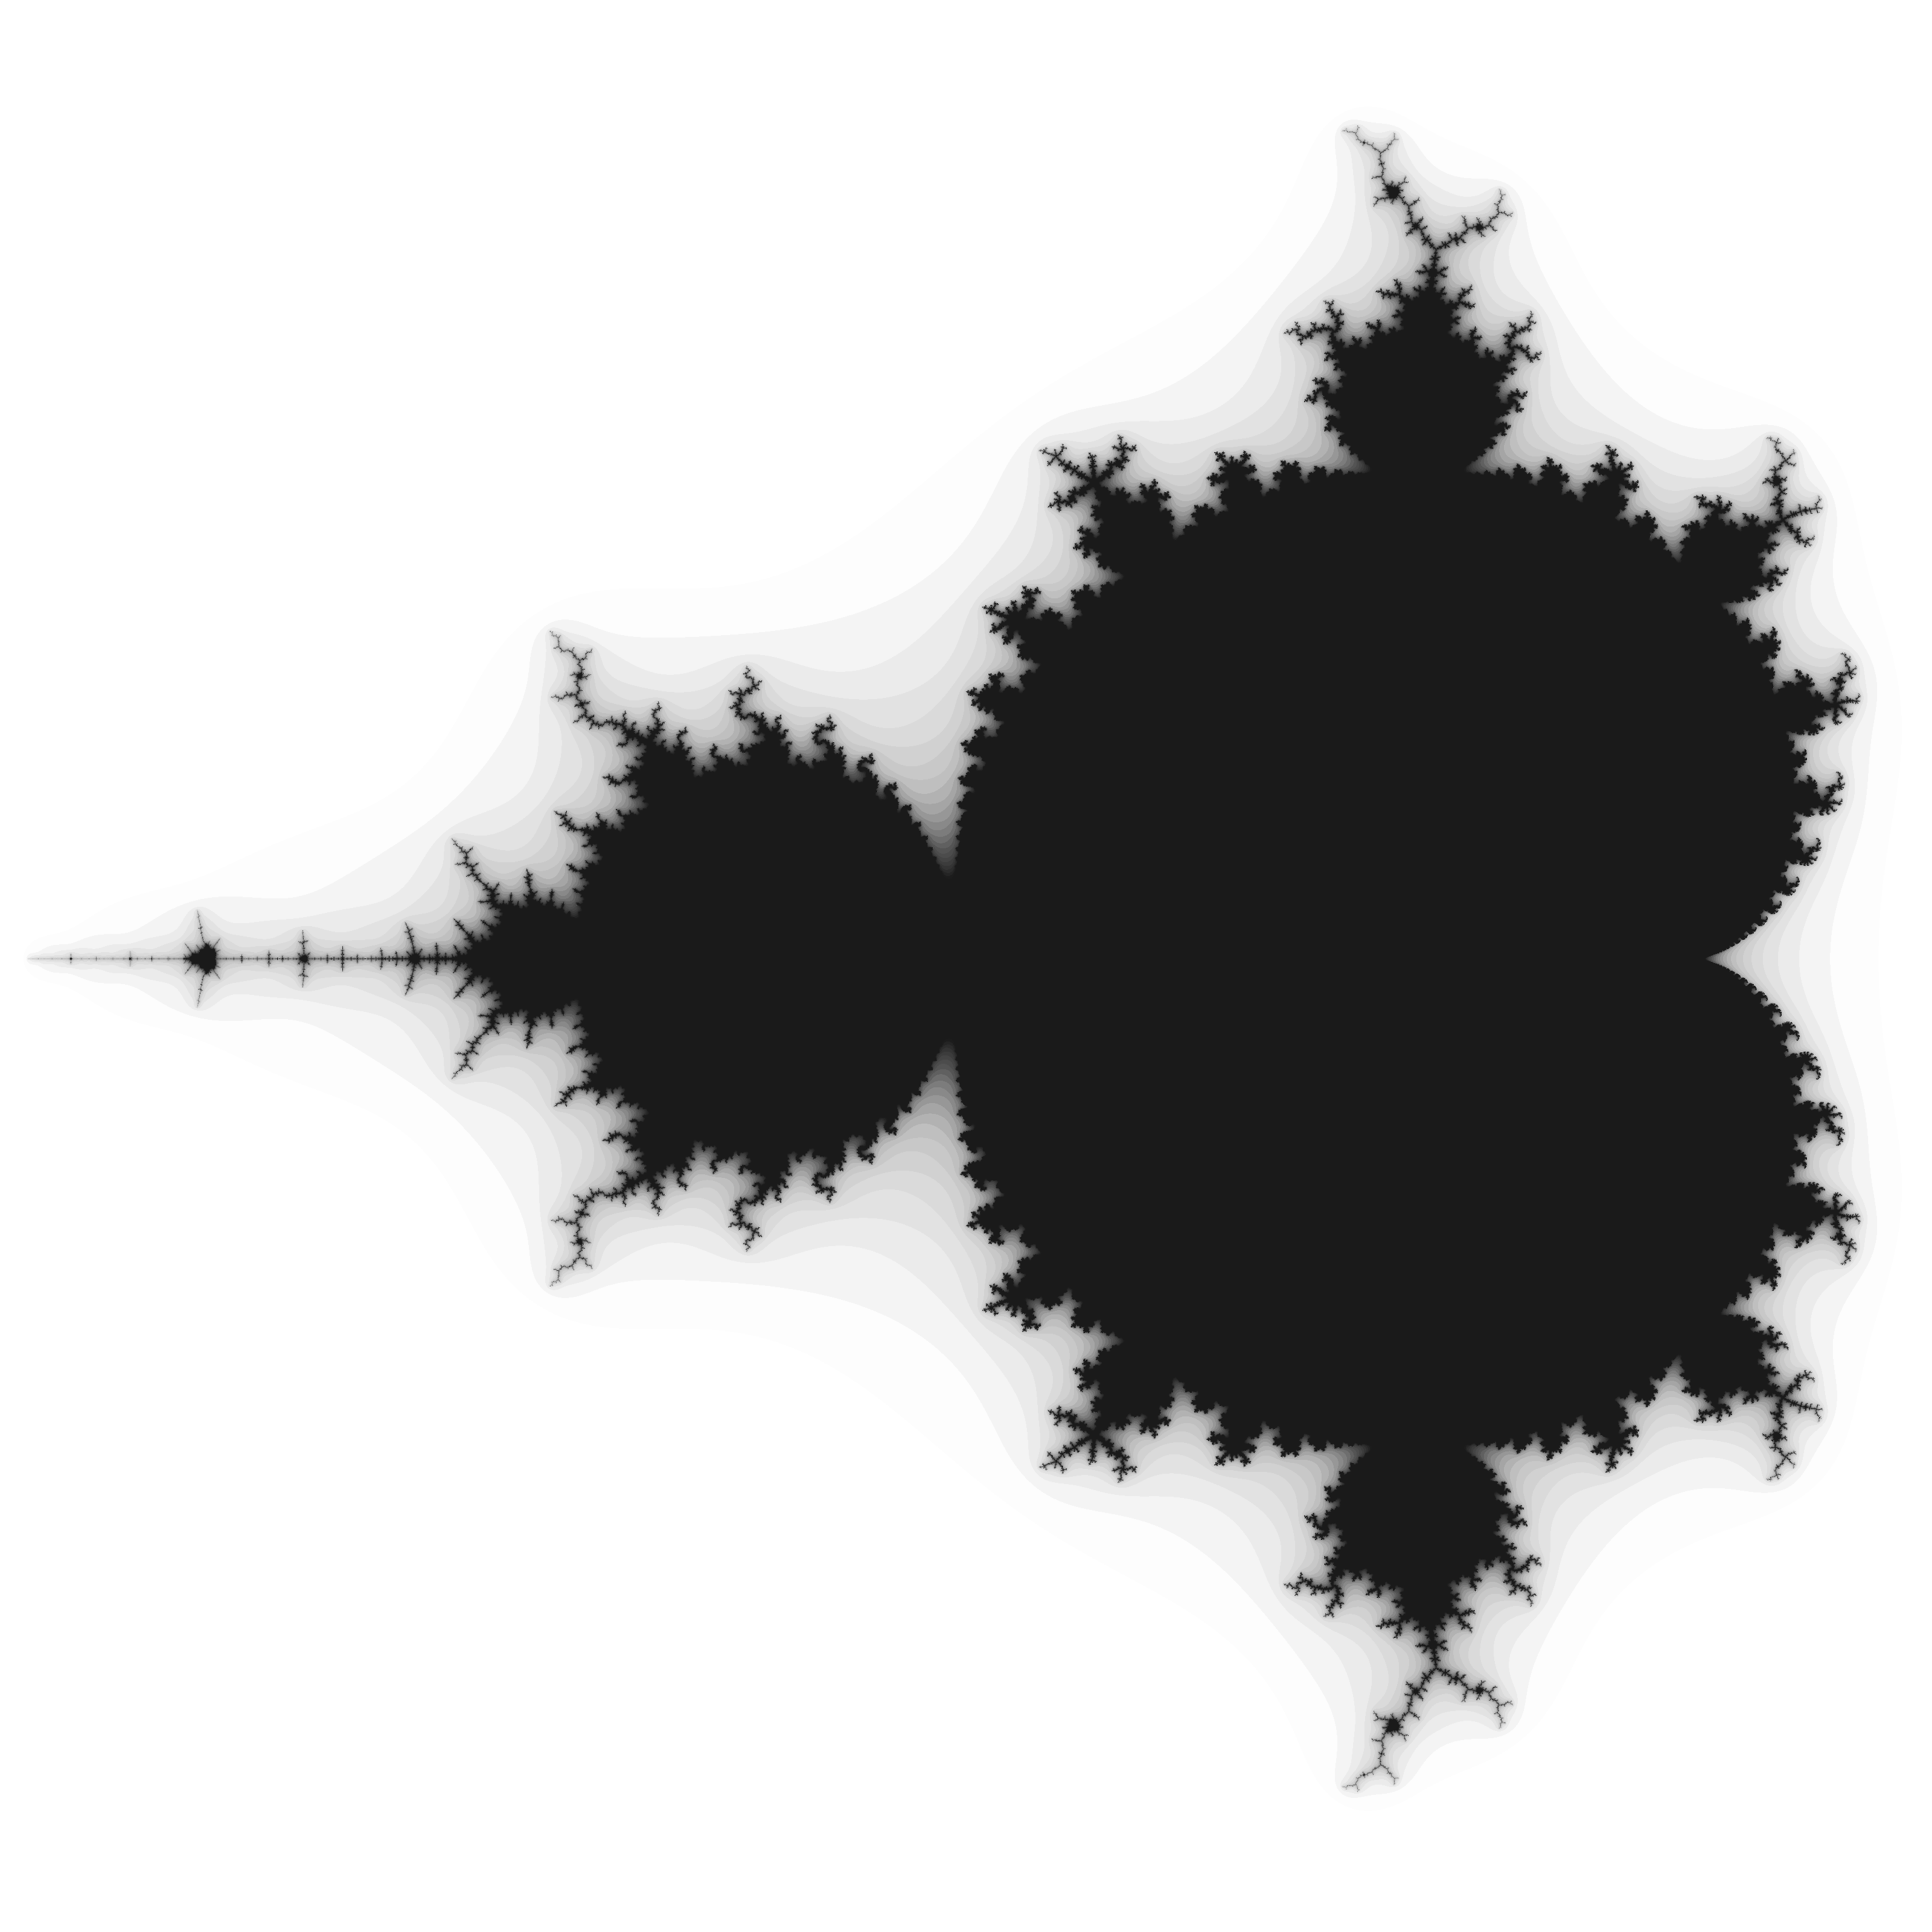
\includegraphics[width=0.6\textwidth]{mandelbrot.png}
\caption{Mandelbrotova množina}
\label{fig:mandelbrot}
\end{figure*}
\section{Úvod}
Fractualiser je program určený pro výkres fraktálů v reálném čase. Umožnujě 
tak uživatelům podbrobně prohlížet jednotlivé části až do přiblížení $10^{13}$
\footnote{Toto omezení je dáno přesností datového typu double, který dokáže
zpracovat GPU. Může se tím pádem lišit mezi počítači.}. Je v něm možné také
právě se zobrazující část fraktálu uložit ve vyšší kvalitě. Bez nastavení je
uložený obrázek čtyřikrát větší, než ten, který je zobrazovaný na obrazovce.
Uživatel ale může tuto hodnotu změnit a fraktál vygenerovat jak velký chce.
Formát uloženého obrázku je Windows Bitmap, také známý pod jeho připonou
\texttt{.bmp}. Implementace Windows Bitmap formátu byla provedena podle
\textcite{bitmapstorage}.

Fractualiser dokáže vykreslovat jen fraktály, které jsou definovány pomocí
jedné funkce v množině komplexních čísel, jako je například Mandelbrotova
množina. Mandelbrotovu množinu definujeme pomocí funkce $f_c(z) = z^2+c$, kde
$z$ a $c$ začínají jako jedno komplexní číslo, o kterém chceme zjistit, zda je
či není v množině. (obrázek \ref{fig:mandelbrot}) Funkci poté provádíme 
opakovaně. Čísla, které nikdy nepřekročí vzdálenost 3 od počátku jsou součástí
množiny.\autocite{mandelbrotwiki}

\subsection{Zadání}
Fractualiser (název složen ze slov fractal a visualiser) je program, který bude
schopen v reálném čase vykreslovat fraktály jako například Mandelbrotovu
množinu, nebo jakoukoliv z Jůliových množin. Uživatel bude moci fraktálem
pohybovat, nebo si jej přiblížit. Program mu také umožní zvýšit počet iterací
pro každý pixel, aby mohl dále klesat do fraktálu. Bude taky schopen uložit
obrázek zrovna zobrazované části fraktálu ve velkém rozlišení. Výpočet a render
bude možné zrychlit pomocí GPU akcelerace.

\subsection{Využité technologie}
Program je napsaný v programovacím jazyce C++. Hlavní důvod využití tohoto
jazyka je jeho rychlost a narozdíl od C jeho podpora objektového programování.
Na vykreslování jsem použil OpenGL API, protože je dobře podporované a
zdokumentované. Dále jsem použil nadstavbu GLFW, která zprostředkovává
zjednodušení a další abstrakce od samotného OpenGL. Na inicializaci OpenGL jsem
použil GLAD. Mi\-mo standardní knihovnu, OpenGL, GLFW a GLAD Fractualiser
nevyužívá žádné jiné kni\-hov\-ny.

Pracoval jsem v editoru NeoVim, přesněji v jeho nadstavbě LunarVim, která
poskytuje plnohodnotné IDE pomocí několika pluginů na analýzu kódu, nebo
debugování přímo v editoru. Jako debugger jsem použil GDB, což je velmi
populární debugger pro Linux, vyvíjen společností Free Software Foundation.
V několika případech byl velmi užitečný. Hlavně když program skončil
chybou SEGFAULT.
